%\section{Luca's Notes}
%
%The usual scenario of ``cold'' natural inflation (NI) is that getting the correct density perturbations requires a flat potential with scale of height much lower than scale of width.
%
%In the natural warm inflation (NWI) scenario, friction means the width of the potential i.e.\ $F$ can be lower than in cold inflation.
%
%Now, as far as the height goes, that would be set by the density perturbations matching CMB. It seems that the height is equally as constrained in the case of thermal fluctuations as it would be in the case of quantum fluctuations.
%
%Effectively, quartic coupling $\lambda < 10^{-10}$ in both cases, where $\lambda = m^2/F^2$. Why is it so, i.e.\ the ratio of height to width of the potential, the same in warm inflation as in cold inflation? I would expect one could get away with a less flat potential in the warm case.
%
%In Minimal Warm Inflation~\cite{Berghaus:2019whh}, on p.12 at the beginning of Section IVA, they say that a single cosine in the case of warm inflation is ruled out. I'm not so sure.  Let us compare your figure 6 in Ref.~\cite{Visinelli:2011jy} against the data following Figure 2 in Will Kinney~\cite{Stein:2021uge}. You can also see the dependence of the natural inflation curves on $F$ in Figure 1 of our older paper~\cite{Freese:2014nla}.
%
%All quantities are in units of the reduced Planck mass $M_{\rm Pl} = 1/\sqrt{8\pi G}$.
%
%We aim to described the evolution of a scalar field $\phi$ coupled with a radiation fluid $R$, for which the equation of motion under a thermodynamical potential $\Omega = \Omega(\phi, T)$ and a damping coefficient $\Gamma = \Gamma(\phi, T)$ is
%\begin{equation}
%	\label{eq:motionphi}
%	\ddot\phi  + (3H+\Gamma)\dot\phi + \Omega_{\phi} = 0\,.
%\end{equation}
%The total energy and pressure of the system is
%\begin{eqnarray}
%	\rho &=& \frac{1}{2}\dot\phi^2 + \Omega + T\,s\,,\\
%	p &=& \frac{1}{2}\dot\phi^2 - \Omega\,,
%\end{eqnarray}
%where the entropy density that ensures the conversion of the inflaton into radiation is $s = -\Omega_{T}$. The effective inflaton potential is~\cite{Weinberg:1974hy, Linde:1978px, Hall:2003zp}
%\begin{equation}
%	\Omega = V(\phi) - p_r\,,
%\end{equation}
%where $p_r = \rho_r/3 = (\pi^2/90)g_*T^4$ and where $s_{\phi} = 0$ when temperature can be neglected with respect to the inflaton mass~\cite{Moss:2006gt} and allows to describe the system in terms of a scalar field and the radiation fluid separately. The conservation of energy-momentum in the form $\dot\rho + 3H (p+\rho) = 0$ together with Eq.~\eqref{eq:motionphi} leads to
%\begin{equation}
%    \label{eq:motionR}
%	\dot\rho_r + 4H \rho_r = W\,,
%\end{equation}
%with the source term $W = \Gamma \dot\phi^2$. Introducing $Q \equiv \Gamma/(3H)$, the slow-roll parameters are
%\begin{eqnarray}
%    \epsilon &\equiv& \frac{1}{2}\left(\frac{V_\phi}{V}\right)^2\,,\\
%    \eta &\equiv& \frac{V_{\phi\phi}}{V}\,,\\
%    \beta &\equiv& \frac{\Gamma_\phi V_\phi}{\Gamma V}\,,
%\end{eqnarray}
%During the slow-roll regime the equations of motion are simplified as
%\begin{eqnarray}
%	\dot\phi &\simeq& -\frac{V_{\phi}}{3H(1+Q)}\,,\label{eq:motionphi_SR}\\
%	\rho_r &\simeq& \frac{3}{4}Q\dot\phi^2\,,\label{eq:motionR_SR}
%\end{eqnarray}
%provided that the slow-roll conditions are satisfied.
%
%We now define three regimes where $H \gtrsim T$ (cold), $H \lesssim T$ and $Q \lesssim 1$ (warm, weak),  $H \lesssim T$ and $Q \gtrsim 1$ (warm, strong). Note, that the Hubble rate is obtained from the expression $H^2 =3\rho$, or from solving
%\begin{equation}
%    H^2 = 3V\left(1 + \frac{1}{18}\frac{2 + 3 Q}{(1 + Q)^2}\frac{\epsilon\, V}{H^2}\right)\,.
%\end{equation}
%Both in the cold and warm regimes, we obtain $H^2 = 3V$ at the lowest order in $Q$ and $\epsilon$.
%
%One useful parametrization in terms of the number of $e$-folds reads
%\begin{equation}
%    N \equiv \int {\rm d}t\,H = -\int {\rm d}\phi\,\frac{1+Q}{\sqrt{2\epsilon}}\,,
%\end{equation}
%so that Eqs.~\eqref{eq:motionphi_SR}-\eqref{eq:motionR_SR} read
%\begin{eqnarray}
%	\phi' &\simeq& -\frac{\sqrt{2\epsilon}}{1+Q}\,,\label{eq:motionphi_SR1}\\
%	\rho_r &\simeq& \frac{Q\epsilon}{2(1+Q)^2} V\,,\label{eq:motionR_SR1}
%\end{eqnarray}
%
%The value of the temperature can be found from the definition for $\rho_r = (\pi^2/30)g_*T^4$ plus the sphaleron decay rate
%\begin{equation}
%    \Gamma = \frac{N_c^5 \alpha_s^5}{2} \frac{T^3}{f^2}\,,
%\end{equation}
%so that Eq.~\eqref{eq:motionR_SR1} gives
%\begin{equation}
%    T = 
%    \begin{cases}
%        \frac{15}{2\pi^2 g}\frac{N_c^5 \alpha^5}{f^2} \epsilon\sqrt{\frac{V}{3}}, &\hbox{\rm weak}\,, \\
%        \left(\frac{30\sqrt{3}}{\pi^2 g} \frac{f^2}{N_c^5 \alpha^5}\, \epsilon\, V^{3/2}\right)^{1/7}, &\hbox{\rm strong}\,,
%    \end{cases}
%\end{equation}
%
%
%
%
%
%The equation of motion for the inflaton field $\phi$ when a friction term $\Gamma$ is included reads
%\begin{equation}
%	\ddot \phi + \left(3H+\Gamma\right)\dot \phi + \frac{\partial}{\partial \phi}V_{\rm eff}(\phi) = 0\,,
%\end{equation}
%where a dot stands for a derivation with respect to cosmic time $t$, a prime means a derivation with respect to the field $\phi$, and the Hubble rate is expressed in terms of the reduced Planck mass $M_{\rm Pl}$ as
%\begin{equation}
%	H = \frac{1}{\sqrt{3}M_{\rm Pl}}\left(\frac{1}{2}\dot\phi^2 +V_{\rm eff}(\phi, T) \right)^{1/2}\,.
%\end{equation}
%
%
%
%Axion potential
%\begin{equation}
%	\mathcal{L} \supset \frac{\alpha}{16\pi}\frac{\phi}{F}G^{\mu\nu}\tilde G_{\mu\nu} - \frac{1}{2}m_0^2\phi^2\,,
%\end{equation}
%so that the mass square is
%\begin{equation}
%	m^2 = m_0^2 + m^2(T)\,,
%\end{equation}
%with $m^2(T) \sim T_c^4/F^2$ for $T \ll T_c$ and $m^2(T) \sim T_c^4/F^2 (T_c/T)^X$ for $T \gg T_c$. At high temperatures we need
%\begin{equation}
%	m_0 \ll (T_c^2/F) (T_c/T)^{X/2}
%\end{equation}
%or $T \ll T_c^{1+4/X}/(m_0F)^{2/X}$.\\
%
%%	m_0 \ll (T_c^2/F) (T_c/H_I)^{X/2}
%
%-----------------------------------
%{\bf Dimensionless equations}
%-----------------------------------
%
%Dimensionless Potential
%\begin{equation}
%    \label{eq:potentialdimensionless}
%    V(\phi) = 1+\cos\phi\,,
%\end{equation}
%Slow-roll equation rescaled
%\begin{eqnarray}
%    3 H (1 + Q) \dot \phi &=& -\frac{{\rm d}V}{{\rm d}\phi}\,,\\
%    H &=& \frac{f}{\sqrt{3}M_{\rm Pl}}\left[\frac{1}{2} \left(1 + \frac{3Q}{2}\right) \dot\phi^2 + V(\phi)\right]^{1/2}\,,
%\end{eqnarray}
%where the potential is in Eq.~\eqref{eq:potentialdimensionless}, $H$ and $\phi$ are dimensionless as $\phi \to \phi/f$, $t \to m_\phi t$ so $H \to H/m_\phi$. Also, $M_{\rm Pl}$ is the reduced Planck mass.
%
%Eq.4.4 in 1106.0701 as a function of $z = k/(aH)$:
%\begin{eqnarray}
%    &&(1 - \epsilon)^2 z^2 y'' - \left(2 + 3 Q (1 - \epsilon) -2 \epsilon (1 - \eta + 2 \epsilon)\right) z y' + (z^2 + 3 \eta (1 + Q) - 3 m Q \frac{\dot\phi}{H \phi}) y = \frac{z^{3/2}}{H^2} \xi - 3 c Q w\,,\\
%    &&(1 - \epsilon) z w' - (4 - c) w = -\frac{z^2}{3 Q} u + 2 (1 - \epsilon) z y'\,,\\
%    && (1 - \epsilon) z u' - 3 (1 + z^2 \zeta) u = 3 Q \left(\frac{w}{3} + y\right)\,,
%\end{eqnarray}
%
%\cite{Ramos:2013nsa}
\section{Perturbations}
\subsection{Background notes}


Our starting point is the perturbed FLRW metric. Following the notation of (CITE: 1106.0701), the metric takes the form
\begin{align}
    ds^2 = -(1+2\alpha)dt^2 - 2 a(t) \partial_i\beta dx^i dt + a^2(t)\left[ (1+2\varphi)\delta_{ij} + 2\partial_i\partial_j \gamma \right]dx^i dx^j.
\end{align}
Here, $a(t)$ is the scale factor, and we consider only the scalar perturbations, denoted by $\alpha$, $\beta$, and $\gamma$. From these, we construct the gauge-invariant metric perturbations:
\begin{align}
    \mathcal{A} &\equiv \alpha - \frac{d}{dt}\left(\frac{\varphi}{H}\right)\\
    \Phi &\equiv \varphi - aH(\beta + a\dot\gamma).
\end{align}
Additionally, we also have fluctuations in the inflaton and radiation sectors. Denoting the inflaton fluctuation as $\delta\phi$ and the radiation energy density and momentum fluctuations as $\delta\rho_r$ and $\Psi_r$, respectively, we construct the gauge-invariant field fluctuations:
\begin{align}
    \delta\phi^{GI} &\equiv \delta\phi - \frac{\dot\phi}{H}\varphi\\
    \delta\rho_r^{GI} &\equiv \delta\rho_r - \frac{\dot\rho_r}{H}\varphi\\
    \Psi_r^{GI} &\equiv \Psi_r - \frac{\rho_r(1+w_r)}{H}\varphi.
\end{align}
The background radiation equation of state parameter $w_r$ can be well-approximated as $w_r \approx 1/3$ for a radiation fluid in near-thermal equilibrium. Taking the dissipation rate to be of the form
\begin{align}
    \Gamma = C_\phi \frac{T^c}{\phi^m},
\end{align}
where $C_\phi$ is a dimensionless constant, the corresponding fluctuation is then
\begin{align}
    \delta\Gamma = \Gamma \left( c\frac{\delta T}{T} - m\frac{\delta\phi}{\phi} \right).
\end{align}
% Since the background radiation source term is given by $\Gamma\dot\phi^2$, we can then express the radiation source fluctuation as
% \begin{align}
%     \delta S_r = \delta\Gamma\dot\phi^2 + 2\Gamma\dot\phi\delta\dot\phi - 2\alpha\Gamma\dot\phi^2,
% \end{align}
% where the last term comes from fluctuations in the fluid four-velocity due to the metric perturbations.

The (Fourier space) gauge-invariant equations of motion then take the form
\begin{align}
    \delta\ddot\phi^{GI} + (3H+\Gamma)\delta\dot\phi^{GI} + \left( \frac{k^2}{a^2} + V_{,\phi\phi} \right)\delta\phi^{GI}
    &= (2\Gamma_{eff}T)^{1/2}a^{-3/2}\xi_k\\
    &- \dot\phi\delta\Gamma^{GI} + \Gamma\dot\phi\mathcal{A} + \dot\phi\dot{\mathcal{A}} + 2(\ddot\phi + 3H\dot\phi)\mathcal{A} - \frac{k^2}{a^2}\dot\phi\frac{\Phi}{H}\\
    \delta\dot\rho_r^{GI} + 3H(1+w_r)\delta\rho_r^{GI}
    &= \frac{k^2}{a^2}\Psi_r^{GI} + (\delta\Gamma\dot\phi^2 + 2\Gamma\dot\phi\delta\dot\phi - 2\alpha\Gamma\dot\phi^2)^{GI} + \dot\rho_r \mathcal{A}\\
    \dot\Psi_r^{GI} + 3H\Psi_r^{GI}
    &= -w_r \delta\rho_r^{GI} - \Gamma\dot\phi\delta\phi^{GI} - \rho_r (1+w_r)\mathcal{A},
\end{align}
where the effective dissipation rate is given by $\Gamma_{eff} = \Gamma + H$. We note that the gauge-invariant metric fluctuation $\mathcal{A}$ vanishes to zeroth order in the slow-roll parameter $\epsilon_H$. This can be seen in its relation to the gauge-invariant comoving curvature perturbation, $\mathcal{R}$:
\begin{align}
    \mathcal{A} = -\frac{\dot H}{H^2}\mathcal{R}.
\end{align}
Likewise, the dissipation rate fluctuation can be expressed to zeroth order in slow-roll as
\begin{align}
    \delta\Gamma^{GI} = \Gamma\left( \frac{c}{3Q\dot\phi^2}\delta\rho_r^{GI} - \frac{m}{\phi}\delta\phi^{GI} \right),
\end{align}
where we have assumed the background radiation bath is in thermal equilibrium. Neglecting other slow-roll suppressed terms and defining the rescaled perturbations,
\begin{align}
    y_k \equiv \frac{k^{3/2}\delta\phi^{GI}}{(2\Gamma_{eff}T)^{1/2}}, \quad w_k \equiv \frac{k^{3/2}\delta\rho_r^{GI}}{(2\Gamma_{eff}T)^{1/2}\Gamma\dot\phi}, \quad u_k \equiv \frac{k^{3/2}\Psi_r^{GI}}{(2\Gamma_{eff}T)^{1/2}\dot\phi},
\end{align}
we can express the equations of motion as
\begin{align}
    \ddot y_k + 3H(1+Q)\dot y_k + H^2 z^2 y_k &= (Hz) ^{3/2}\xi_k - 3cQH^2 w_k\\
    \dot w_k + (4-c)H w_k &= \frac{H}{3Q}z^2 u_k + 2\dot y_k\\
    \dot u_k + 3H u_k &= -QH(w_k + 3y_k).
\end{align}
Here, we define the dimensionless dissipation rate $Q \equiv \Gamma/(3H)$ and the redshift time coordinate $z \equiv k/(aH)$. 


\section{Luca's notes}

\subsection{Equations for the perturbations}

We consider the equations for the perturbations in warm inflation in the Newtonian gauge, where the metric is
\begin{equation}
    {\rm d}s^2 = -(1 - 2\varphi){\rm d}t^2 - 2 a(t) \partial_i\beta dx^i dt + a^2(t)\left[ (1+2\varphi)\delta_{ij} + 2\partial_i\partial_j \gamma \right]{\rm d}x^i {\rm d}x^j\,,
\end{equation}
where the perturbation terms $\beta$, $\gamma$ and $\varphi$ are space-time dependent. In the Newtonian gauge, the gauge-invariant quantity $\chi \equiv a(\beta + a\dot\gamma) = 0$. Since $\beta$ and $\gamma$ enter the expressions for the scalar perturbations only through the term $\chi$, we can safely set $\beta = \gamma = 0$. We assume that the friction term $\Gamma = \Gamma(T, \phi)$ is given as
\begin{align}
    \Gamma = C_\phi \frac{T^c}{M_{\rm Pl}^a\,\phi^m},
\end{align}
where $C_\phi$ is a dimensionless constant with $c-a-m=1$, so that the corresponding fluctuation is
\begin{align}
    \delta\Gamma = \Gamma \left( c\frac{\delta T}{T} - m\frac{\delta\phi}{\phi} \right) \approx \Gamma \left( c\frac{\delta \rho_r}{4\rho_r} - m\frac{\delta\phi}{\phi} \right)\,,
\end{align}
where in the last step we assumed that the fluctuations in the temperature are related to the radiation density perturbations as
\begin{equation}
	\frac{\delta T}{T} \approx \frac{\delta \rho_r}{4\rho_r}\,.
\end{equation}
The perturbation of the source term $W = \Gamma \dot\phi^2$ in the Newtonian gauge reads~\cite{Das:2020xmh, Bastero-Gil:2011rva}
\begin{equation}
	\delta W \equiv \delta\Gamma \dot\phi^2 + 2\Gamma\dot\phi\delta\dot\phi + 2\varphi\Gamma\dot\phi^2 =  \Gamma \left[\left(\frac{c}{4}\frac{\delta \rho_r}{\rho_r} - m \frac{\delta\phi}{\phi}\right) \dot\phi^2 + 2\dot\phi\delta\dot\phi + 2\varphi\dot\phi^2\right]\,.
\end{equation}
In momentum space, the equation of motion for the fluctuations with comoving wavenumber ${\bf k}$ at zeroth-order in the slow-roll parameters is given by~\cite{Kodama:1984ziu, Hwang:1991aj, Hwang:2001fb, Malik:2002jb}
\begin{eqnarray}
    \delta\dot \rho_r + \left(4 H - \frac{3 c Q}{4}\frac{\dot\phi^2}{\rho_r}\right) \delta\rho_r &=& \frac{k^2}{a^2} \Psi + 3H Q \dot\phi^2\left(\varphi + 2 \frac{\delta\dot\phi}{\dot\phi} - m \frac{\delta\phi}{\phi}\right) + 4 \rho_r \left(\frac{1}{2 M_{\rm Pl}^2}\left(\dot\phi\delta\phi - \Psi\right) + H \varphi\right)\,,\label{eq:fluctuationsR}\\
	\dot\Psi + 3H\Psi &=& - \frac{1}{3}\delta\rho_r - 3QH\dot\phi\delta\phi + \frac{4}{3}\rho_r\varphi\,.\label{eq:fluctuationsPsi}
\end{eqnarray}
At the same time, the field fluctuations $\delta \phi = \delta \phi({\bf x}, t)$ are described by a stochastic Langevin equation~\cite{Moss:2007cv, Graham:2009bf},
\begin{equation}
	\label{eq:fluctuations}
	\delta\ddot\phi + 3H(1+Q) \delta\dot\phi - \frac{1}{a^2}\nabla^2\delta\phi = \Gamma_{\rm eff}\,\xi({\bf x}, t) - \frac{cH}{\dot\phi}\delta\rho_r\,,
\end{equation}
$$\delta\ddot\phi + 3 H (1 + Q) \delta\dot\phi + \left(\frac{k^2}{a^2} + V_{\phi\phi} - 3 m H Q \frac{\dot\phi}{\phi}\right) \delta\phi = \Gamma_{\rm eff}\,\xi_T - \frac{cH}{\dot\phi} \delta\rho_r + \dot\phi\left(\frac{2}{M_{\rm Pl}^2}(\dot\phi \delta\phi - \Psi) + H \varphi\right) + (3 H (1 + Q) \dot\phi + 2 V_\phi) \varphi\,,$$
where $\Gamma_{\rm eff} = [2(\Gamma+H)T]^{1/2}$ and the noise term $\xi({\bf x}, t)$ satisfies~\cite{Berera:2007qm}
\begin{equation}
	\label{eq:correlation}
	\langle\xi({\bf x}, t); \xi({\bf x'}, t') \rangle = (2\pi)^3\,a^{-3}\delta^{(3)}({\bf x}-{\bf x'})\delta(t-t')\,.
\end{equation}
We take the Fourier transform of Eq.~\eqref{eq:fluctuations} as
\begin{equation}
	\delta\phi({\bf x}, t) = \int {\rm d}^3{\bf k}\,e^{i {\bf k}\cdot{\bf x}} \,\delta\phi({\bf k}, t)
\end{equation}
Care is needed when rewriting the noise correlation in Eq.~\eqref{eq:correlation}. We express $\delta(t-t')$ in terms of redshift $z$ using the relation $Ht =-\ln(Hz/k)$, so that
\begin{equation}
	\delta(t-t') = H\delta\left(\ln\left(\frac{k z'}{k' z}\right)\right) = Hz \,\delta\left(z - z'\frac{k}{k'}\right)\,,
\end{equation}
so that the Fourier transform of Eq.~\eqref{eq:correlation} with $a^{-3} = (Hz/k)^3$ is
\begin{equation}
	\label{eq:correlation1}
	\langle\xi({\bf k}, z); \xi({\bf k'}, z') \rangle = (2\pi)^3\,\frac{H^4z^4}{k^3} \delta^{(3)}({\bf k} + {\bf k'})\delta(z - z')\,.
\end{equation}
The Fourier transform of the field fluctuations follows the expression
\begin{equation}
	\label{eq:fluctuations1}
	\delta\ddot\phi + 3H(1+Q) \delta\dot\phi + \frac{k^2}{a^2}\nabla^2\delta\phi = \Gamma_{\rm eff}\,\frac{H^2z^2}{k^{3/2}}\hat\xi({\bf k}, z) - \frac{cH}{\dot\phi}\delta\rho_r\,,
\end{equation}
where we have introduced the rescaled Gaussian noise term $\hat\xi({\bf k}, z)$ of mean zero and standard deviation one, satisfying the correlation
\begin{equation}
	\label{eq:correlation2}
	\langle\hat\xi({\bf k}, z); \hat\xi({\bf k'}, z') \rangle = (2\pi)^3\, \delta^{(3)}({\bf k} + {\bf k'})\delta(z - z')\,.
\end{equation}
We switch to the variables
\begin{eqnarray}
	y_k &=& \frac{k^{3/2}}{\Gamma_{\rm eff}}\delta\phi\,,\\
	w_k &=& \frac{k^{3/2}}{\Gamma_{\rm eff}(\Gamma\dot\phi)}\delta\rho_r\,,\\
	u_k &=& \frac{k^{3/2}}{\Gamma_{\rm eff}\dot\phi}\Psi\,,	
\end{eqnarray}
in terms of which Eqs.~\eqref{eq:fluctuationsR},~\eqref{eq:fluctuationsPsi} and~\eqref{eq:fluctuations1} read
\begin{eqnarray}
	\ddot y_k + 3H(1+Q) \dot y_k + H^2\left(z^2 - 3 m Q \frac{\dot\phi}{H \phi}\right)y_k &=& H^2z^2 \hat\xi({\bf k}, z) - 3cQH^2w_k\,,\label{eq:fluctuationsphi1}\\
	\dot w_k + (4-c)H w_k &=& \frac{k^2}{a^2}\frac{u_k}{3QH} - m \frac{\dot\phi}{\phi} y_k + 2\dot y_k\,,\label{eq:fluctuationsR1}\\
	\dot u_k + 3H\left(1+z^2\zeta\right)u_k &=& - QHw_k - 3QHy_k\,.\label{eq:fluctuationsPsi1}
\end{eqnarray}
We switch to the independent variable $z = k/(aH)$ to obtain the set of differential equations,
\begin{eqnarray}
	y_k'' - \frac{2+3Q}{z}y_k' + \left(1 + \frac{3 m Q}{z^2} \frac{z\phi'}{\phi}\right)y_k &=& \hat\xi({\bf k}, z) - \frac{3cQ}{z^2}w_k\,,\label{eq:fluctuationsphi2}\\
	zw_k' - (4-c)w_k &=& -\frac{z^2}{3Q}u_k - m \frac{z\phi'}{\phi} y_k + 2zy_k'\,,\label{eq:fluctuationsR2}\\
	zu_k' - 3\left(1+z^2\zeta\right)u_k &=& Q\left(w_k + 3y_k\right)\,.\label{eq:fluctuationsPsi2}
\end{eqnarray}
The set of equations is solved starting well inside horizon $z_0 \gg 1$ with initial conditions $y_k(z_0) = 1$, $y_k'(z_0)= 0$, $w_k(z_0) = 0$, and $u_k(z_0) = 0$.

\subsection{Numerical solution}

We introduce the variable $\tau = \ln z$ and we write $x_k = y_k'$, so that the system of Eqs.~\eqref{eq:fluctuationsphi2}--\eqref{eq:fluctuationsR2} is
\begin{eqnarray}
	\frac{{\rm d}x_k}{{\rm d}\tau} &=& 3(1+Q)x_k - \left(z^2 + \frac{3mQ}{\phi}\frac{{\rm d}\phi}{{\rm d}\tau}\right)y_k - 3cQw_k + z^{3/2}\tilde\xi({\bf k}, \tau)\,,\label{eq:fluctuationsphi3}\\
	\frac{{\rm d}y_k}{{\rm d}\tau} &=& x_k\,,\\
	\frac{{\rm d}w_k}{{\rm d}\tau} &=& (4-c)w_k - \frac{z^2}{3}\tilde u_k - \frac{m}{\phi}\frac{{\rm d}\phi}{{\rm d}\tau} y_k + 2x_k\,,\label{eq:fluctuationsR3}\\
	\frac{{\rm d}\tilde u_k}{{\rm d}\tau} &=& 3\left(1+z^2\zeta\right)\tilde u_k + w_k + 3y_k\,,\label{eq:fluctuationsPsi3}
\end{eqnarray}
where $\tilde\xi({\bf k}, \tau) = z^{1/2}\hat\xi({\bf k}, z)$ and $\tilde u_k = u_k/Q$. With this set of equations we are able to solve for the function $y_k$.

For $m\neq 0$, the equations above have to be coupled with the expression for the background
\begin{equation}
    \frac{V_\phi}{M_{\rm Pl}^2} (1 + Q) \frac{{\rm d}\phi}{{\rm d}\tau} = V(\phi)\,,  
\end{equation}
where $M_{\rm Pl} = 1/\sqrt{8\pi G}$ is the the reduced Planck mass. Setting the inflaton potential as
\begin{eqnarray}
    V(\phi) &=& m_\phi^2 f^2\left[1-\cos(\phi/f)\right]\,, \\   
    V_\phi(\phi) &=& m_\phi^2 f\sin(\phi/f)\,,    
\end{eqnarray}
we obtain the expression for the background
\begin{equation}
    \left(\frac{f}{M_{\rm Pl}}\right)^2\,(1 + Q)\,\frac{{\rm d}(\phi/f)}{{\rm d}\tau} =  \frac{\sin(\phi/f)}{1-\cos(\phi/f)}\,. 
\end{equation}
The result can be expressed in quadrature, with solution
\begin{equation}
    \phi= 2 f \arcsin\left[\sin\left(\frac{\phi_i}{2f}\right)\sqrt{\exp\left(\frac{1}{1 + Q}\left(\frac{M_{\rm Pl}}{f}\right)^2(\tau - \tau_i)\right)}\right]\,.
\end{equation}





The relation with the observations come by considering the dimensionless primordial curvature power spectrum that include friction effects,
\begin{equation}
    \label{eq:PS}
    \Delta_{\mathcal{R}}^{2}=\left(\frac{H^{2}}{2 \pi \dot{\phi}}\right)^{2}\left(1 + 2 n_{\mathrm{BE}}+\frac{2 \sqrt{3} \pi Q}{\sqrt{3+4 \pi Q}} \frac{T}{H}\right) G(Q)\,,
\end{equation}
where the quantities are all evaluated at horizon crossing and $n_{\mathrm{BE}} = [\exp(H/T )-1]^{-1}$ is the Bose-Einstein distribution function. We consider the strong limit of warm inflation, for which $T \gtrsim H$, so that $1+2n_{\mathrm{BE}} \approx 2T/H$ which can be neglected in Eq.~\eqref{eq:PS} when $Q \gtrsim 1$.

For a choice of the parameters $c$ and $Q$, we perform a series of simulations $y_k^{(i)}$, where $i \in \{1... N_{\rm run}\}$ and where $N_{\rm run}$ is the total number of simulations. We build the realization
\begin{equation}
    \langle y_k^2 \rangle \equiv \sum_i (y_k^{(i)})^2\,,
\end{equation}
where the sum is taken over the number of simulations, so that the amplitude of the primordial spectrum is expressed in terms of the inflaton field as~\cite{Bastero-Gil:2011rva}
\begin{equation}
    \label{eq:basterogil}
	\Delta_{\mathcal{R}}^{2} = \left(\frac{H}{\dot\phi}\right)^2\,\frac{\Gamma_{\rm eff}^2}{2\pi^2}\,\langle y_k^2\rangle_* = 4(3Q+1)\left(\frac{H^2}{2\pi\dot\phi}\right)^2\,\frac{T}{H}\,\langle y_k^2\rangle_*\,,
\end{equation}
where the star indicates that the quantity is evaluated at horizon crossing. Comparing the results in Eq.~\eqref{eq:PS} and~\eqref{eq:basterogil} gives
\begin{equation}
    \label{eq:comparison}
    G(Q) = 2 (3 Q + 1 ) \frac{\sqrt{3 + 4 \pi Q}}{\sqrt{3} \pi Q}\,\langle y_k^2\rangle_*\,.
\end{equation}
Starting from Eq.~\eqref{eq:comparison}, the results in Ref.~\cite{Bastero-Gil:2011rva} can then be cast as
\begin{equation}
    G_{\rm Bastero-Gil}(Q) = \frac{\sqrt{3 + 4 \pi Q}}{\sqrt{3} \pi Q}\,\frac{\sqrt{3\pi}}{2}\sqrt{Q+1}\,\left(A_cQ^\alpha+B_cQ^\beta\right)\,,
\end{equation}
where for $c = 1$ they find $A_c = 2.8\times 10^{-2}$, $B_c = 6.8 \times 10^{-5}$, $\alpha = 2.5$ and $\beta = 2.0$. The results in Ref.~\cite{Benetti:2016jhf} are
\begin{equation}
    G_{\rm Benetti}(Q) = 1 + A_cQ^\alpha+B_cQ^\beta\,,
\end{equation}
where for $c =1$ they find $A_c = 0.335$, $B_c = 0.0185$, $\alpha = 1.364$ and $\beta = 2.315$. 

While we reproduce the results in Ref.~\cite{Bastero-Gil:2011rva} for the range of friction terms considered in that paper, we find that it is not possible to extrapolate the fitting function they provide for values $Q\gtrsim 10^3$. For this, we have extended the fit by considering the function
\begin{eqnarray}
	G(Q) &=& 2 (3 Q + 1 ) \frac{\sqrt{3 + 4 \pi Q}}{\sqrt{3} \pi Q}\,10^{F(\log_{10}Q)}\,,\\
	F(x) &=& a_0 +a_1 x + a_2 x^2 + a_3 x^3\,.
\end{eqnarray}
The results for the fit are given in Table~\ref{tabParams}.

\begin{table}[hb]
\def\arraystretch{1.5}
	\begin{tabular}{ccccc}
    \hline\hline
		$c$ & $a_0$ & $a_1$ & $a_2$ & $a_3$ \\
		\hline
		3 & 1.4885 & -0.1550 & 2.2262 & -0.1811 \\ 
		1 & -0.0202 & 0.5100 & 0.6280 & -0.0529 \\
		\hline
	\end{tabular}
	\caption{Fitting coefficients}
	\label{tabParams}
\end{table}


\begin{figure}
    \centering
    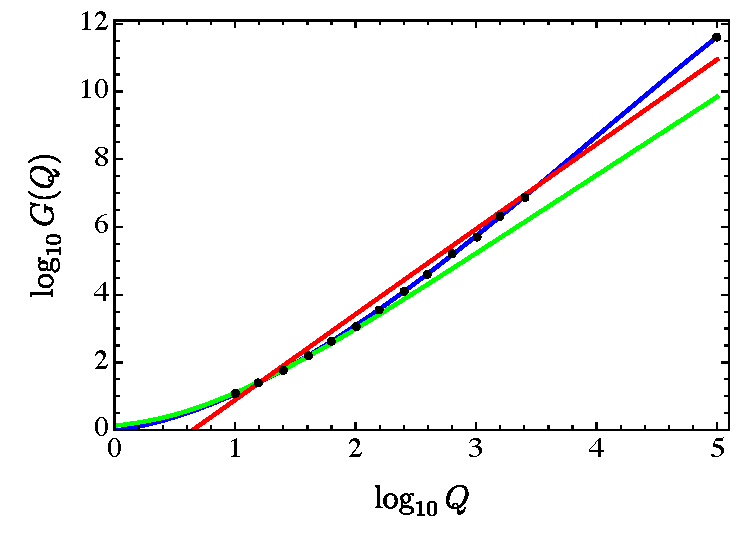
\includegraphics[width=0.7\linewidth]{plotc1.pdf}
    \caption{The function $G(Q)$ for Ref.~\cite{Bastero-Gil:2011rva} (red), Ref.~\cite{Benetti:2016jhf} (green), and our fit (blue) to the numerical results obtained (black dots).}
    \label{fig:GQc1}
\end{figure}



\section{Limit $Q\gg1$}
In the limit $Q \gg 1$ the second order derivative in Eq.~\eqref{eq:fluctuationsphi2} can be neglected since $y_k'' \sim y_k/z^2 \ll y_k/z_F^2$, so that we obtain
\begin{equation}
	\label{eq:fluctuationsphi3}
	- \frac{3Q}{z}y_k' = -y_k + \hat\xi({\bf k}, z) - \frac{3cQ}{z^2}w_k\,.
\end{equation}
Inserting this expression into Eq.~\eqref{eq:fluctuationsR2} in the limit $Q \gg 1$ greatly simplifies the expression for $w_k$ as there are various cancellations leading to
\begin{equation}
	\label{eq:fluctuationsR3}
	w_k'' - \frac{8-c}{z}w_k'+\frac{1}{3}w_k + y_k  = 0\,.
\end{equation}

If we neglect the higher-order derivatives for the same reason as above, then for $z \gg 1$ the solution for $w_k$ tracks $y_k$ as $w_k  = -3y_k$ and Eq.~\eqref{eq:fluctuationsphi3} reads
\begin{equation}
	\label{eq:fluctuationsphi4}
	\frac{{\rm d}y_k}{{\rm d}x} = 3x\left(\frac{1}{2}- \frac{c}{x^2}\right) y_k - \frac{3}{2}x \hat\xi({\bf k}, z)\,.
\end{equation}
where $x \equiv z/z_F$ and $z_F = 3(Q/2)^{1/2}$. We are interested in solving the equation with the initial condition $y_k = y_0$ starting from $x_0 \gg 1$ and evaluating it at $x = 1$ (or $z = z_F$). This is a linear stochastic differential equation, so that if $\hat\xi({\bf k}, z)$ is Gaussian distributed at $x_0 \gg 1$, the same applies at $x = 1$ with the mean $\mu$ and standard deviation $V$ given by respectively by
\begin{eqnarray}
	\frac{{\rm d}\mu}{{\rm d}x} &=& 3x\left(\frac{1}{2}- \frac{c}{x^2}\right)\mu\,,\\
	\frac{{\rm d}V}{{\rm d}x} &=& 6x\left(\frac{1}{2}- \frac{c}{x^2}\right)V + \frac{9}{4}x^2\,,
\end{eqnarray}
with solution
\begin{eqnarray}
	\mu &=& y_0 \left(\frac{x}{x_0}\right)^{-3 c} \exp\left(\frac{3}{4}(x^2 - x_0^2)\right)\,,\\
	V &=& \frac{1}{2}\left(\frac{3}{2}\right)^{\frac{1 - 6 c}{2}} e^{\frac{3}{2} x^2} x^{-6 c}\Gamma\left(\frac{3}{2} + 3 c, \frac{3}{2} x^2\right)\,.
\end{eqnarray}
In particular, for $x = 1$ the mean is zero while we obtain the variance at freezeout ($x = 1$):
\begin{equation}
	V = \frac{1}{2}\left(\frac{3}{2}\right)^{\frac{1 - 6 c}{2}} e^{3/2}\Gamma\left(\frac{3}{2} + 3 c, \frac{3}{2}\right)\,.
\end{equation}
As expected, this solution is independent on the initial conditions, but also on the value of $Q$ and gives $V \approx 80900$ for $c = 3$ and $V\approx 9.1$ for $c = 1$. This is in contrast with the results in Fig.3 of Ref.~\cite{Bastero-Gil:2011rva}, however a numerical solution of Eqs.~\eqref{eq:fluctuationsphi2}--\eqref{eq:fluctuationsR2} shows that the approximation in Eq.~\eqref{eq:fluctuationsphi4} is correct for large values of $Q$.

%The perturbations over the radiation energy density follow the expression~\cite{Graham:2009bf}
%\begin{equation}
%	\label{eq:fluctuationsR}
%	\delta\ddot \rho_r + 9 H \delta\dot \rho_r + \left(20 H^2 + \frac{1}{3}\frac{k^2}{a^2}\right) \delta\rho_r = \frac{k^2}{a^2} J + 5 H\delta W + \delta \dot W\,,
%\end{equation}
%where $\delta W$ and $J$ represent the transfer of energy and momentum into the radiation bath, respectively, as~\cite{Moss:2006gt,Moss:2007cv}
%\begin{equation}
%	\delta W = \dot\phi^2\delta\Gamma\,,\qquad J = -\Gamma\dot\phi\delta\phi\,.
%\end{equation}
%Here, the inflaton field has been decomposed as
%\begin{equation}
%	\phi({\bf x}, t) \to \phi(t) + \delta\phi({\bf x}, t)\,,
%\end{equation}
%where the evolution of the background field $\phi(t)$ on super-horizon scales does not depend on the spatial coordinates. 
%
%We do not include the dependence on $\phi$ so that $\delta \Gamma = \Gamma_T \delta T$ and $\delta W = c H \delta\rho_r$, so that
%\begin{equation}
%	\delta\ddot \rho_r + (9 - c)H \delta\dot \rho_r + \left((20-5c) H^2 + \frac{1}{3}\frac{k^2}{a^2}\right) \delta\rho_r = -\frac{k^2}{a^2}\Gamma\dot\phi\delta\phi\,.
%\end{equation}
%At the zeroth order in the variable $z = k/(aH)$, with $\delta\dot\phi = -H z \delta\phi'$ and $\delta\ddot\phi = H^2 z^2 \delta\phi'' + H^2 z \delta\phi'$ with the prime being the derivation with respect to $z$ gives
%\begin{equation}
%	\label{eq:fluctuationsR2}
%	\delta\rho_r'' - \frac{8 - c}{z}\delta\rho_r' + \left(\frac{20-5c}{z^2} + \frac{1}{3}\right) \delta\rho_r = -\frac{1}{z^2}\Gamma\dot\phi\delta\phi\,.
%\end{equation}
%
%
%We decompose the field of fluctuations in Fourier modes according to
%\begin{equation}
%	\delta\phi({\bf x}, t) = \frac{1}{(2\pi)^3}\int{\rm d}^3 {\bf k}\, e^{i {\bf k}\cdot{\bf x}}\,\delta\phi({\bf k}, t)\,,
%\end{equation}
%and we switch to the independent variable $z$ so that
%\begin{equation}
%	\label{eq:fluctuations2}
%	\delta\phi'' - \frac{2 + 3Q}{z} \delta\phi' + \delta\phi + \frac{3cQ}{z^2} (\Gamma\dot\phi)^{-1}\delta\rho_r = \frac{\Gamma_{\rm eff}}{H^2z^2}\,\xi\,.
%\end{equation}
%Eqs.~\eqref{eq:fluctuationsR2}--\eqref{eq:fluctuations2} with the independent variables 
%\begin{equation}
%	y_k = k^{3/2}\frac{\delta\phi}{\Gamma_{\rm eff}}\,,\qquad w_k = k^{3/2}\frac{\delta\rho_r}{\Gamma_{\rm eff}\gamma\dot\phi}\,,
%\end{equation}
%gives
%\begin{eqnarray}
%	w_k'' - \frac{8 - c}{z}w_k' + \left(\frac{20-5c}{z^2} + \frac{1}{3}\right) w_k + y_k &=& 0\,,\\
%	y_k'' - \frac{2 + 3Q}{z} y_k' + y_k + \frac{3cQ}{z^2} w_k &=& \hat\xi\,,
%\end{eqnarray}
%where the noise term $\hat\xi({\bf k}, t)$ satisfies
%\begin{equation}
%	\langle\xi({\bf k}, t)\xi({\bf k'}, t') \rangle = (2\pi)^3\,\delta^{(3)}({\bf k}-{\bf k'})\delta(t-t')\,.
%\end{equation}
%

\section{Including the background}

\begin{eqnarray}
    \ddot\phi+3H(1+Q)\dot\phi+V_\phi &=& 0\,,\label{eq:phi}\\
    \dot\rho_r + 4H\rho_r &=& 3HQ\dot\phi^2\,,\label{eq:rhoR}\\
    H^2 &=& \frac{1}{3M_{\rm Pl}^2}\left(\frac{1}{2}\dot\phi^2 + V(\phi) + \rho_r\right)\,.
\end{eqnarray}
We define $z =k/(aH)$ and we introduce the slow-roll parameters
\begin{eqnarray}
    \epsilon_H &\equiv& -\frac{\dot H}{H^2}\,,\label{def_epsilonH}\\
    \eta_H &\equiv& \frac{1}{H}\frac{{\rm d}\ln\epsilon_H}{{\rm d}t} = \frac{\ddot H}{H \dot H} + 2\epsilon_H\,,
\end{eqnarray}
so that $\ddot H = H^3\epsilon_H(2\epsilon_H-\eta_H)$. We introduce $\tau = \ln z$ and $b \equiv \ln \phi/f$, so that
\begin{eqnarray}
    \frac{1}{\phi}\dot \phi &=& \frac{\dot z}{z} b'\,,\\
    \frac{1}{\phi}\ddot \phi &=& \left(\frac{\dot z}{z}\right)^2(b')^2 + \frac{\ddot z}{z}b' - \left(\frac{\dot z}{z}\right)^2b' + \left(\frac{\dot z}{z}\right)^2b''\,,
\end{eqnarray}
or, since $\dot z = -Hz(1-\epsilon_H)$ and $\ddot z = H^2z(1-\epsilon_H+\epsilon_H\eta_H)$, we obtain
\begin{eqnarray}
    \frac{1}{\phi}\dot \phi &=& -H(1-\epsilon_H) b'\,,\\
    \frac{1}{\phi}\ddot \phi &=& H^2(1-\epsilon_H)^2(b')^2 + H^2\epsilon_H(1-\epsilon_H+\eta_H)b' + H^2(1-\epsilon_H)^2b''\,.
\end{eqnarray}
This gives
\begin{equation}
    \label{eq:phiEQM}
    (1-\epsilon_H)^2[b''+(b')^2] - [3(1+Q)(1-\epsilon_H)-\epsilon_H(1-\epsilon_H+\eta_H)]b' + \frac{1}{H^2}\frac{V_\phi}{\phi} = 0\,.
\end{equation}
Finally, the Hubble rate and its derivative are
\begin{eqnarray}
    H^2 &=& \frac{1}{3M_{\rm Pl}^2}\left(\frac{1}{2}\dot\phi^2 + V + \rho_r\right)\,,\label{eq:H2}\\
    \dot H &=& -\frac{1}{2M_{\rm Pl}^2}\left(\frac{4}{3}\rho_r + \dot\phi^2\right)\,,\label{eq:Hdot}\\
    \ddot H &=& \frac{1}{M_{\rm Pl}^2}\left(\frac{8}{3}H\rho_r + H(3+Q)\dot\phi^2+\dot\phi\,V_\phi\right)\,.
\end{eqnarray}

We rescale the potential as $V = m_\phi^2f^2 \tilde V$, along with $\tilde \rho_r = \rho_r/(f^2m_\phi^2)$ and $\tilde H = H/m_\phi$, so that we obtain a system of equations
\begin{eqnarray}
    \tilde H^2 &=& \frac{\tilde f^2}{3}\left[\frac{1}{2}\tilde H^2(1-\epsilon_H)^2e^{2b}(b')^2 + \tilde V + \tilde \rho_r\right]\,,\label{eq:tildeH}\\
    \epsilon_H\,\tilde H^2 &=& \tilde f^2\left[\frac{1}{2}\tilde H^2(1-\epsilon_H)^2e^{2b}(b')^2 + \frac{2}{3}\tilde\rho_r\right]\,,\label{eq:epsilonH1}
\end{eqnarray}
where the Hubble rate and the slow-roll parameter $\epsilon_H$ appear on both sides of the equations, with $\tilde f = f/M_{\rm Pl}$. The system of Eqs.~\eqref{eq:tildeH}--\eqref{eq:epsilonH1} can be solved explicitly to give
\begin{eqnarray}
    \tilde H^2 &=& \frac{\tilde f^2}{6 - 4(b')^2 e^{2b}\tilde f^2}\bigg\{V \!+\! \rho_r \!-\! 2(b')^2 e^{2 b} \tilde f^2\left(V+\frac{1}{3}\rho_r \right) \!+\! \left[(V+\rho_r)^2\left(1 - \frac{2}{3}(b')^2 e^{2 b} \tilde f^2\right) \!+\! \frac{8}{3}V^2(b')^2 e^{2 b} \tilde f^2\right]^{1/2}\!\bigg\}\,,\label{def:H2}\\
    \dot {\tilde H} &=& -\frac{\tilde H^2}{(b')^2e^{2b}\tilde f^2}\left[1+(b')^2e^{2 b}\tilde f^2 - \sqrt{1 + 2(b')^2 e^{2 b} \tilde f^2 \left(1 - \frac{2}{3}\frac{\tilde f^2}{\tilde H^2} \tilde\rho_r\right)} \right]\,,\label{def:Hdot}\\
    \ddot{\tilde H} &=& \tilde H \tilde f^2 \left(\frac{8}{3}\tilde \rho_r + {\tilde H}^2 (3+Q)(1-\epsilon_H)^2 e^{2b}(b')^2 - (1-\epsilon_H) e^b b'\,\tilde V_\phi\right)\,.
\end{eqnarray}
This way, the only parameters left are the value of $\tilde f$ and of the initial condition of the inflaton field, which we set at $\phi = f$ or $b = 0$. The limits of the expressions for $b' \to 0$ and $\rho_r \to 0$ reduce to the expected expressions in Eqs.~\eqref{eq:H2}-\eqref{eq:Hdot} in the slow-roll limit. The slow-roll parameter has the simple form
\begin{equation}
    \epsilon_H = 3 - \frac{\tilde f^2}{\tilde H^2}\left(\tilde V+\frac{1}{3}\tilde\rho_r\right)\,,
\end{equation}
and the condition $\epsilon_H = 1$ for the end of inflation is achieved when $V = 2\dot\phi^2 +\rho_r$.

We now have the tools to write down the expressions for the background in terms of the 


solve Eqs.~\eqref{eq:phi}-\eqref{eq:rhoR} written as the system:
\begin{eqnarray}
    b' &=& b_1\,,\\
    b_1' &=& - b_1^2 + \frac{1}{(1-\epsilon_H)^2}\bigg\{[3(1+Q)(1-\epsilon_H)-\epsilon_H(1-\epsilon_H+\eta_H)]b_1 - \frac{1}{\tilde H^2}\frac{1}{\tilde\phi}\frac{{\rm d}\tilde V}{{\rm d}\tilde\phi}\bigg\} \,,\\
    \tilde \rho_r' &=& 4\tilde \rho_r - 3Q \tilde H^2(1-\epsilon_H)^2 (b')^2e^{2b}\,,
\end{eqnarray}
along with the expressions in Eqs.~\eqref{def:H2}-\eqref{def:Hdot}.

Note, that the relation between cosmic time and $\tau$ can be obtained from the expression
\begin{equation}
    \frac{{\rm d}\tau}{{\rm d}t} = - H - \frac{\dot H}{H}\,,
\end{equation}
which is obtained by differentiating the definition for $z$.


 where $m_\phi^2 = \lambda f^2/4$ for the quartic potential.

\begin{eqnarray}
    \tilde V &=& 1-\cos(\phi/f) = 1 - \cos e^b\,,\\
    \tilde V_\phi &=& \sin e^b\,,
\end{eqnarray}
and with the rescaling
so that the last term in Eq.~\eqref{eq:phiEQM} in these two forms reads respectively
\begin{equation}
    \label{eq:Vcases}
    \frac{V_\phi}{\phi} =
    \begin{cases}
        \lambda f^2\,e^{2b}\qquad &\hbox{(Quadratic)}\,,\\
        m_\phi^2\,e^{-b}\,\sin e^b\qquad &\hbox{(Cosine)}\,.
    \end{cases}
\end{equation}



We consider the following shapes for the potential:
\begin{align}
    V(\phi) &= \frac{\lambda}{4}\phi^4, \quad & \hbox{(Quadratic)}\,,\\
    V(\phi) &= m_\phi^2f^2\left[1-\cos(\phi/f)\right], \quad & \hbox{(Cosine)}\,,
\end{align}
and 




\clearpage
\section{Gab's Notes: perturbations with background using Newtonian's slicing}
\subsection{Perturbation equations}
Following the notation in \cite{Das:2020xmh}, the perturbation equations read:
\begin{align}
\delta \ddot{\phi}=&-3 H(1+Q) \delta \dot{\phi}-\left(\frac{k^2}{a^2}+V_{, \phi \phi}-\frac{3m H Q \dot{\phi}}{\phi}\right) \delta \phi \nonumber \\+& \xi_q+\xi_T-\frac{c H}{\dot{\phi}} \delta \rho_r+\dot{\phi}(\kappa+\dot{\alpha})+[2 \ddot{\phi}+3 H(1+Q) \dot{\phi}] \alpha, \label{eq:Gab1} \\ \delta \dot{\rho}_r=&-H\left(4-\frac{3 c Q \dot{\phi}^2}{4 \rho_r}\right) \delta \rho_r+\frac{k^2}{a^2} \Psi_r+6 H Q \dot{\phi} \delta \dot{\phi} \nonumber\\ &-\frac{3m H Q \dot{\phi}^2}{\phi} \delta \phi+\frac{4 \rho_r}{3} \kappa-3 H\left(Q \dot{\phi}^2+\frac{4 \rho_r}{3}\right) \alpha, \label{eq:Gab2}\\ \dot{\Psi}_r=&-3 H \Psi_r-3 H Q \dot{\phi} \delta \phi-\frac{1}{3} \delta \rho_r-4 \rho_r \frac{\alpha}{3} . \label{eq:Gab3}\\
 \kappa &=\frac{3}{2 M_{\mathrm{Pl}}^2}\left(\dot{\phi} \delta \phi-\Psi_r\right), \label{eq:Gab4} \\ \alpha &=-\varphi,\label{eq:Gab5} \\ \dot{\varphi} &=-H \varphi-\frac{1}{3} \kappa . \label{eq:Gab6}
 \end{align}
where the stochastic thermal and quantum sources $\xi_T$ and $\xi_q$ can be approximated by a localized Gaussian distribution with correlation function:
\begin{align}
    \left\langle\xi_T(t, x) \xi_T\left(t^{\prime}, x^{\prime}\right)\right\rangle&=(2\pi)^3\frac{2\Gamma T}{ a^3}\delta\left(t-t^{\prime}\right) \delta^{(3)}\left(x-x^{\prime}\right), \\
    \left\langle\xi_q(t, x) \xi_q\left(t^{\prime}, x^{\prime}\right)\right\rangle&=(2\pi)^3\frac{H^2\sqrt{9+12\pi Q}}{ \pi a^3}\cdot(1+2n_{\mathrm{EB}})\delta\left(t-t^{\prime}\right) \delta^{(3)}\left(x-x^{\prime}\right),    
\end{align}
with $\Upsilon(\phi, T)=C_{\Upsilon} M^{1-c+m} T^c/ \phi^m$ and $n_{\mathrm{EB}}=\frac{1}{e^{H/T}-1}$.

The metric perturbation equations really correspond to two constraints equations (Eqs.\ref{eq:Gab4} and \ref{eq:Gab5}) and one dynamic equation (Eq.\ref{eq:Gab6}). Therefore we will simply substitute Eqs.\ref{eq:Gab4} and \ref{eq:Gab5} in the other 4 equations of motion. Doing so, the equation for $\varphi$ becomes:
\begin{equation}
  \dot{\varphi} =-H \varphi- \frac{1}{2 M_{\mathrm{Pl}}^2}\left(\dot{\phi} \delta \phi-\Psi_r\right),
\end{equation}

We will now perform a change of variable from $t\rightarrow \tau$ where $\tau=\ln z$ and $z=k/(aH)$. It can be easily shown that for any function $f(t)$ it follows:
\begin{align}
    \dot{f}&=H(\epsilon_H-1)f^\prime, \\
    \ddot{f}&=H^2(\epsilon_H-1)^2 f^{\prime\prime}+H^2(\epsilon_H+\epsilon_H\eta_H-\epsilon_H^2)f^\prime,
\end{align}
where $\dot{}=d/dt$, $^\prime=d/d\tau$ and:
\begin{align}
    \epsilon_H=-\frac{\dot{H}}{H^2}; \quad \eta_H=\frac{1}{H}\frac{d\ln\epsilon_H}{dt}.
\end{align}
We will also reparameterize all of the dynamical variables by $k^{3/2}$ and rescale the thermal noise such that:
\begin{align}
&\{\delta\hat{\phi},\delta\hat{\rho}_r,\hat{\Psi}_r,\hat{\varphi}\}=k^{-3/2}\{\delta\phi,\delta\rho_r,\Psi_r,\varphi\}, \\
& \xi_T(\vec{x},t)\rightarrow \frac{\Xi_T H^2e^{3\tau/2}}{k^{3/2}}\hat{\xi}_T(\vec{k},\tau),\\
& \xi_q(\vec{x},t)\rightarrow \frac{\Xi_{\mathrm{q}}H^2e^{3\tau/2}}{k^{3/2}}\hat{\xi}_q(\vec{k},\tau),\\
&\langle\hat{\xi}_T(\vec{k},\tau) \hat{\xi}_T(\vec{k}^\prime,\tau^\prime)\rangle=(2\pi)^3\delta\left(\tau-\tau^{\prime}\right) \delta^{(3)}(\vec{k}-\vec{k}^{\prime}),\\
&\langle\hat{\xi}_q(\vec{k},\tau) \hat{\xi}_q(\vec{k}^\prime,\tau^\prime)\rangle=(2\pi)^3\delta\left(\tau-\tau^{\prime}\right) \delta^{(3)}(\vec{k}-\vec{k}^{\prime});
\end{align}
where $\Xi_{\mathrm{q}}\equiv \frac{H(9+12\pi Q)^{1/4}}{ \sqrt{\pi}}\sqrt{1+2n_{\mathrm{EB}}}$ and $\Xi_T\equiv 2\Gamma T$.

Putting all of this together, our perturbation equations finally become:
\begin{align}
    (1-\epsilon_H)^2\delta \hat{\phi}^{\prime\prime}&+\epsilon_H(1+\eta_H-\epsilon_H)\delta\hat{\phi}^\prime=3 (1+Q)(1-\epsilon_H) \delta \hat{\phi}^\prime-\left(e^{2\tau}+\frac{V_{, \phi \phi}}{H^2}-\frac{3mQ \dot{\phi}}{\phi H}\right) \delta \hat{\phi} \nonumber \\+& \Xi_T e^{3\tau/2}\hat{\xi}_T+\Xi_q e^{3\tau/2}\hat{\xi}_q-\frac{c}{\dot{\phi}H} \delta \rho_r+\frac{\dot{\phi}}{H^2}\left[\frac{2}{ M_{\mathrm{Pl}}^2}\left(\dot{\phi} \delta \hat{\phi}-\hat{\Psi}_r\right)+H\hat{\varphi}\right]+[2 \ddot{\phi}-3 H(1+Q) \dot{\phi}]\frac{ \hat{\varphi}}{H^2}, \label{eq:Gab2.1} \\ (1-\epsilon_H)\delta \hat{\rho}^\prime_r=&\left(4-\frac{3c Q \dot{\phi}^2}{4 \rho_r}\right) \delta \hat{\rho_r}-He^{2\tau}\hat{\Psi}_r+6 H Q (1-\epsilon_H)\dot{\phi} \delta \hat{\phi}^\prime \nonumber\\ &+\frac{3m Q \dot{\phi}^2}{\phi} \delta \hat{\phi}-\frac{2 \rho_r}{ H M_{\mathrm{Pl}}^2} \left(\dot{\phi} \delta \hat{\phi}-\hat{\Psi}_r\right)-3\left(Q \dot{\phi}^2+\frac{4 \rho_r}{3}\right) \hat{\varphi}, \label{eq:Gab2.2}\\ (1-\epsilon_H)\hat{\Psi}^\prime_r=&3 \hat{\Psi}_r+3Q \dot{\phi} \delta \hat{\phi}+\frac{1}{3H} \delta \hat{\rho}_r-4 \rho_r \frac{\hat{\varphi}}{3H}, \label{eq:Gab2.3} \\
      (1-\epsilon_H)\hat{\varphi}^\prime& = \hat{\varphi}+ \frac{1}{2H M_{\mathrm{Pl}}^2}\left(\dot{\phi} \delta \hat{\phi}-\hat{\Psi}_r\right). \label{eq:Gab2.4}
\end{align}
This system of equations can be solved numerically subject to the initial conditions: $\{\hat{\phi}_0,\hat{\phi}^\prime_0,\hat{\rho}^0_r,\hat{\Psi}^0_r,\hat{\varphi}_0\}$ and for known background evolution of: $\{H,\epsilon_H,\eta_H,Q,T,\phi,\dot{\phi},\ddot{\phi}\}$.

With this parametrization the scalar power spectrum is given by:
\begin{equation}
    \Delta_{\mathcal{R}}(k)=\frac{1}{2 \pi^2}\left\langle|\hat{\mathcal{R}}|^2\right\rangle,
\end{equation}
where:
\begin{align}
    \hat{\mathcal{R}}&=\sum_{i=\phi, r} \frac{\rho_i+\bar{p}_i}{\rho+\bar{p}} \hat{\mathcal{R}}_i, \\
    \hat{\mathcal{R}}_i&=-\hat{\varphi}-\frac{H}{\rho_i+\bar{p}_i} \hat{\Psi}_i,
\end{align}
with $\hat{\Psi}_\phi\equiv -\dot{\phi}\delta \hat{\phi}$, $\bar{p}=p_\phi+p_r$, $\bar{p}_\phi \equiv p_\phi=\frac{1}{2}\dot{\phi}^2-V$, $\rho_\phi=\frac{1}{2}\dot{\phi}^2+V$ and $\bar{p}_r\equiv p_r=\frac{1}{3}\rho_r=\frac{\pi^2}{90}g_{*}T^4$.

\subsection{Perturbation equations without metric perturbations and $c=0$}
If we set the metric perturbations to zero and set $c=0$, the full set of perturbation equations becomes:
\begin{align}
\delta \ddot{\phi}=&-3 H(1+Q) \delta \dot{\phi}-\left(\frac{k^2}{a^2}+V_{, \phi \phi}-\frac{3m H Q \dot{\phi}}{\phi}\right) \delta \phi +\xi_q+\xi_T , \label{eq2:Gab1} \\ \delta \dot{\rho}_r=&-4H \delta \rho_r+\frac{k^2}{a^2} \Psi_r+6 H Q \dot{\phi} \delta\dot{\phi}, \label{eq2:Gab2}\\ 
\dot{\Psi}_r=&-3 H \Psi_r-3 H Q \dot{\phi} \delta \phi-\frac{1}{3} \delta \rho_r, \label{eq2:Gab3}
 \end{align}
where we will once again make the assumption that the stochastic thermal and quantum sources $\xi_T$ and $\xi_q$ can be approximated by a localized Gaussian distribution with correlation function:
\begin{align}
    \left\langle\xi_T(t, x) \xi_T\left(t^{\prime}, x^{\prime}\right)\right\rangle&=(2\pi)^3\frac{2\Gamma T}{ a^3}\delta\left(t-t^{\prime}\right) \delta^{(3)}\left(x-x^{\prime}\right), \label{eq:noiseT}\\
    \left\langle\xi_q(t, x) \xi_q\left(t^{\prime}, x^{\prime}\right)\right\rangle&=(2\pi)^3\frac{H^2\sqrt{9+12\pi Q}}{ \pi a^3}\cdot(1+2n_{\mathrm{EB}})\delta\left(t-t^{\prime}\right) \delta^{(3)}\left(x-x^{\prime}\right),  \label{eq:noiseQ}  
\end{align}
with $\Upsilon(\phi, T)=C_{\Upsilon} M^{1-m}/ \phi^m$ and $n_{\mathrm{EB}}=\frac{1}{e^{H/T}-1}$.


We will now perform a change of variable from $t\rightarrow z$ where  $z=k/(aH)$ to zeroth order in the slow-roll coefficients. It can be easily shown that for any function $f(t)$ it follows:
\begin{align}
    \dot{f}=-Hzf^\prime, \quad \ddot{f}=H^2z^2\left(f^{\prime\prime}+\frac{f^\prime}{z}\right),
\end{align}
where $\dot{}=d/dt$, $^\prime=d/d\tau$. 
For $c=0$, we can clearly see in Eq.\ref{eq2:Gab1} that the scalar field perturbations are \textit{decoupled} from the radiation perturbations (both $\delta\rho_R$ and $\Psi_R$). We can rewrite Eq.\ref{eq2:Gab1} as:
\begin{align}
    &H^2z^2\left(\delta \phi^{\prime\prime}+\frac{\delta\phi^\prime}{z}\right)=3H^2z(1+Q)\delta \phi^\prime-\left(z^2H^2+V_{, \phi \phi}-\frac{3mHQ \dot{\phi}}{\phi}\right) \delta \phi +\xi_T+\xi_q, \nonumber \\
    &\delta \phi^{\prime\prime}=\frac{3Q+2}{z}\delta \phi^\prime-\left(1+\frac{V_{, \phi \phi}}{z^2H^2}-\frac{3mQ \dot{\phi}}{z^2 H\phi}\right) \delta \phi +\frac{\xi_T+\xi_q}{z^2H^2}.\label{eq2:Gab4}
\end{align}
This can further recasted as:
\begin{equation}
 \delta \phi^{\prime \prime}-\frac{1}{z}(3 Q+2) \delta \phi^{\prime}+\left[1+3 \frac{\eta_V-\beta_V Q /(1+Q)}{z^2}\right] \delta \phi =\frac{1}{H^2 z^2}\left[\xi_T+\xi_q\right], \label{eq2:Gab5}
\end{equation}
where we used the fact that $\eta_V=M_{\rm{pl}}^2V_{,\phi\phi}/V$ and $\beta_V=M_{\rm{pl}}^2\Upsilon_{,\phi}V_{,\phi}/(\Upsilon V)$ with $M_{\rm{pl}}^2=1$ in our units. 

The general solution to eq.\ref{eq2:Gab5} can be written as:

\begin{equation}
\delta \phi(\mathbf{k}, z)=\int_z^{\infty} d z^{\prime} G\left(z, z^{\prime}\right) \frac{\left(z^{\prime}\right)^{1-2 \nu}}{z^{\prime 2} H^2}\left[\xi_q\left(z^{\prime}\right)+\xi_T\left(z^{\prime}\right)\right],
\end{equation}
where the Green's function $G(z,z^\prime)$ is given in terms of Bessel functions:
\begin{equation}
    G\left(z, z^{\prime}\right)=\frac{\pi}{2} z^\nu z^{\prime \nu}\left[J_\alpha(z) Y_\alpha\left(z^{\prime}\right)-J_\alpha\left(z^{\prime}\right) Y_\alpha(z)\right].
\end{equation}
with $z^\prime>z$ and:
\begin{align}
\nu & =3(1+Q) / 2, \\
\alpha & =\sqrt{\nu^2+\frac{3 \beta
Q}{1+Q}-3 \eta}.
\end{align}
From this we can finally derive the correlation function of the scalar field fluctuations:

\begin{align}
\left\langle\delta \phi(\mathbf{k}, z) \delta \varphi\left(\mathbf{k}^{\prime}, z\right)\right\rangle  &=\frac{1}{H^4} \int_z^{\infty} d z_2 \int_z^{\infty} d z_1 G\left(z, z_1\right) G\left(z, z_2\right) \frac{\left(z_1\right)^{1-2 \nu}}{z_1^2} \frac{\left(z_2\right)^{1-2 \nu}}{z_2^2}\left[\left\langle\xi_q \xi_q\right\rangle +\left\langle\xi_T\xi_T\right\rangle \right] \nonumber \\
\text{(Eqs.\ref{eq:noiseT}+\ref{eq:noiseQ}):} \quad &=\left[\frac{\Upsilon T}{\pi^2}+\frac{H^2\sqrt{9+12\pi Q}}{ 2\pi^3}\cdot(1+2n_{\mathrm{BE}}) \right]\int_z^{\infty} d z^{\prime} z^{\prime 2-4 \nu} G\left(z, z^{\prime}\right)^2 \nonumber \\
 \text{($\eta, \beta \ll 1$, i.e. $\alpha\approx\nu$):} \quad &\approx \left[\frac{\Upsilon T}{16\pi^2}+\frac{H^2\sqrt{9+12\pi Q}}{ 32\pi^3}\cdot(1+2n_{\mathrm{BE}}) \right] \frac{\left[2^\nu \Gamma(\nu)\right]^2 \Gamma(\nu-1)}{\Gamma(2 \nu-1 / 2) \Gamma(\nu-1 / 2)} \nonumber \\
 &\approx \left[\frac{\Upsilon T}{16\pi^2}+\frac{H^2\sqrt{9+12\pi Q}}{ 32\pi^3}\cdot(1+2n_{\mathrm{BE}}) \right]\frac{8\pi}{\sqrt{9+12\pi Q}}\nonumber \\
 &=\frac{H^2}{4\pi^2}\left[1+2n_{\mathrm{BE}}+\frac{T}{H}\frac{2\sqrt{3}\pi Q}{\sqrt{3+4\pi Q}} \right]
\end{align}
where we used the properties of the $\Gamma$ function to obtain the second to last equality and assumed $\Upsilon$, $T$, $H$ and $Q$ to be approximately constant with respect to $z$.

From a perturbed Friedmann-Robertson-Walker metric with spatial curvature perturbation $\psi$, it can be defined a gauge invariant comoving curvature perturbation as $\mathcal{R}(x, t) = \psi(x, t) + H\delta\phi(x, t)/\dot{\phi}$, which remains conserved throughout the evolution on super horizon scales. We can then choose a spatially flat gauge,
and write the curvature perturbation simple as $\mathcal{R}= H\delta\phi/\dot{\phi}$. From this it follows:
\begin{align}
    \Delta_{\mathcal{R}}^2&=\frac{H^2}{\dot{\phi}^2}\Delta_{\phi}^2 \nonumber \\
    &=\left(\frac{H^2}{2\pi \dot{\phi}}\right)\left[1+2n_{\mathrm{BE}}+\frac{T}{H}\frac{2\sqrt{3}\pi Q}{\sqrt{3+4\pi Q}} \right]
\end{align}